\chapter{A Path Towards Calibration of the OVRO-LWA}
\label{chapter2}

\begin{bibunit}

\section{Design and Construction of the OVRO-LWA}

\begin{figure}
    \centering
    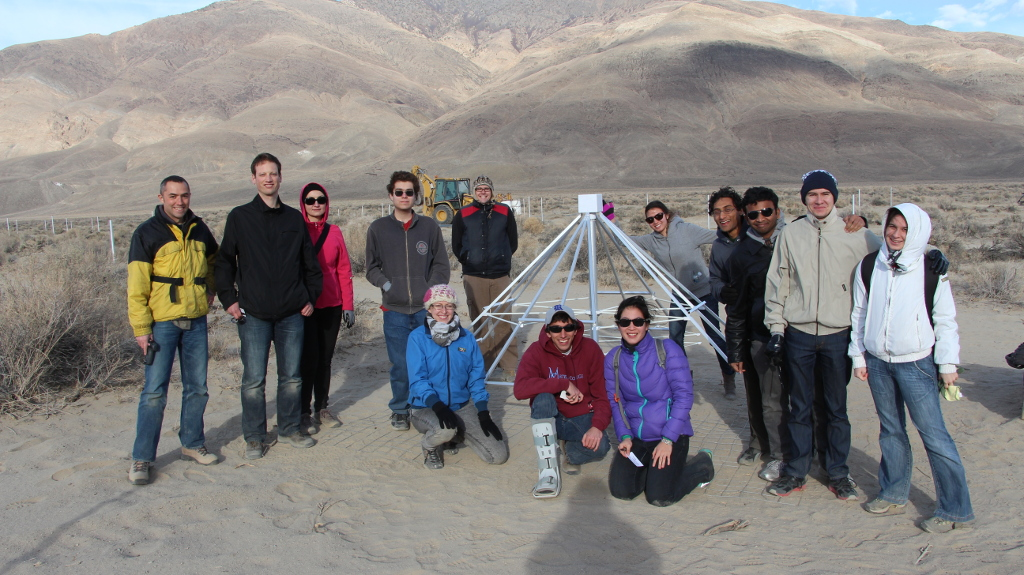
\includegraphics[width=\textwidth]{figures/chapter2/first-antenna}
    \caption{
        The first OVRO-LWA completed on 2013 March 8 with the class of Ay~122b (including the author
        of this thesis with the fractured ankle).
    }
    \label{fig:ovro-first-antenna}
\end{figure}

\begin{figure}
    \centering
    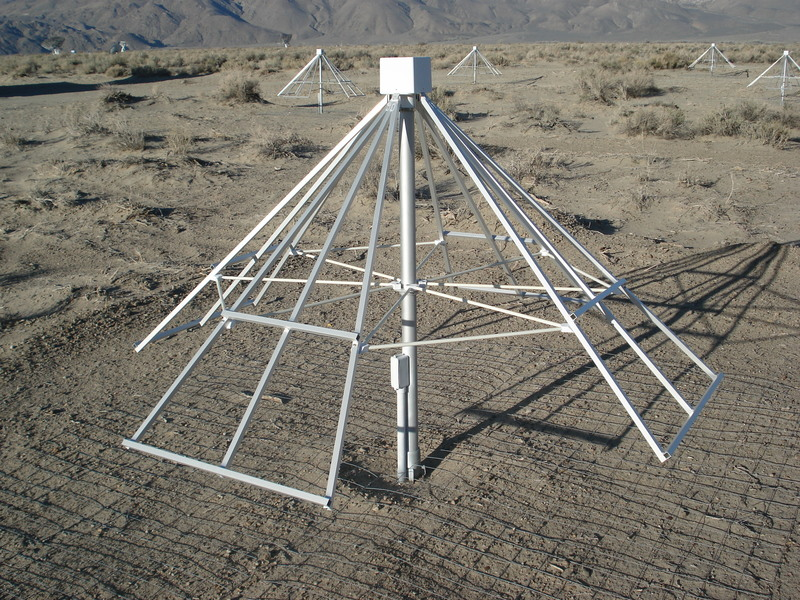
\includegraphics[width=\textwidth]{figures/chapter2/lwa-antenna}
    \caption{
        Picture of an OVRO-LWA antenna.
    }
    \label{fig:ovro-lwa-pictures}
\end{figure}

The OVRO-LWA is a new low-frequency (27--85\,MHz instantaneous) radio interferometer constructed
during the course of this thesis and located near Big Pine, California. Construction began in 2013
with the first antenna completed in March of that year (see Figure~\ref{fig:ovro-first-antenna}).

The OVRO-LWA was initially composed of 256 antennas, with 251 of those antennas arranged within a
dense 200\,m diameter core in a configuration that is optimized for sidelobe levels in snapshot
imaging.  Each of these antennas consists of two crossed broadband dipoles with an active
balun/preamp, and the entire system is sky noise dominated over the range 20--80\,MHz
\citep{2012PASP..124.1090H}.  A picture of an OVRO-LWA antenna can be seen in
Figure~\ref{fig:ovro-lwa-pictures}. The primary beam of each OVRO-LWA antenna subtends a solid angle
of $\sim 8000\,\text{deg}^2$, with sensitivity to the entire visible hemisphere of the sky.

\todo{ARX boards}

The remaining five antennas are isolated from the core of the OVRO-LWA and equipped with radiometric
front ends as part of the LEDA experiment, which is attempting to measure the globally averaged
signal of \ion{H}{1} from the Cosmic Dawn \citep{2018MNRAS.478.4193P}.  The OVRO-LWA hosts the LEDA
correlator as its back-end, which is an FX correlator composed of 16 ROACH2 FPGAs that compose the F
stage, and 11 servers each with dual NVIDIA K20X GPUs that compose the X stage
\citep{2015JAI.....450003K}. This allows the correlator to perform full cross-correlation of 512
input signals with 58\,MHz instantaneous bandwidth.

During observations, data is streamed from the LEDA correlator to the All-Sky Transient Monitor
(ASTM), which houses the compute nodes used for post-processing and imaging.  The ASTM is composed
of 10 identical nodes each with a 16-core Intel Xeon E5-2630 v3 CPU and 64\,GB of memory. Five
additional servers provide 565\,TB of storage capacity through the Lustre high performance file
system.

The initial 256 antenna interferometer was therefore capable of imaging the entire visible
hemisphere in snapshot images with 1$\arcdeg$ angular resolution. An example snapshot image can be
seen in Figure~\ref{fig:core-snapshot-image}.  In 2015, an additional 32 antennas were installed
that extended the maximum baseline of the interferometer to 1.5\,km and improved the angular
resolution to 8$\arcmin$. This improved angular resolution can be seen in
Figure~\ref{fig:expansion-snapshot-image}. In a final future stage of development, an additional 64
antennas will be installed that extend the maximum baseline to 2.6\,km, which will see improved
$uv$-coverage at long baselines and improved $5\arcmin$ angular resolution.

While this thesis focuses on the use of the OVRO-LWA to detect the high-redshift signature of
neutral hydrogen from the Cosmic Dawn, the OVRO-LWA facilitates a diverse set of scientific
motivations including the study of stellar and planetary magnetospheres, radio follow-up of gamma
ray bursts \citep{2017arXiv171106665A} and neutron star mergers, solar dynamic imaging spectroscopy,
and the detection of high energy cosmic rays \citep{caltechthesis11016}.

With the exception of detecting high energy cosmic rays---which uses a custom firmware and
processing pipeline that cannot operate in parallel with ordinary correlation---there are two
complementary software pipelines that service the scientific goals of the OVRO-LWA:
\begin{enumerate}
    \item A widefield snapshot imaging pipeline that images the entire visible hemisphere every
        13\,s using WSCLEAN \citep{2014MNRAS.444..606O}.
    \item A novel approach specialized for drift-scanning interferometers that can image the entire
        sky (above a limiting declination) in a single synthesis imaging step.
\end{enumerate}
This chapter will describe the calibration, source removal routines purpose built for the OVRO-LWA
and used by both pipelines. Additionally, in \S\ref{sec:commissioning-challenges} I will discuss
some of the challenges involved with commissioning the OVRO-LWA that have been overcome to bring the
OVRO-LWA into existence, to first light, and finally its first scientific results.  Finally, the
latter pipeline will be discussed in considerable depth in Chapters~\ref{chapter3} and
\ref{chapter4}.

\begin{figure}[p]
    \centering
    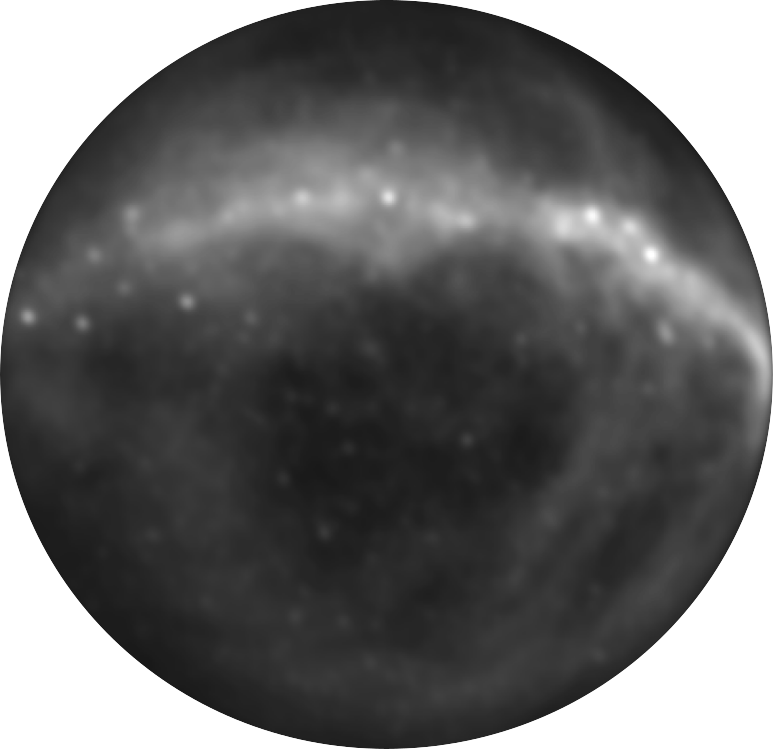
\includegraphics[width=\textwidth]{figures/chapter2/before-expansion}
    \caption{
        Snapshot image of the sky captured with the OVRO-LWA and using only the antennas located
        within the core of the array. The image covers the entire visible hemisphere in
        sine-projection.  A similar image constructed using the newer long-baseline antennas can be
        seen in Figure~\ref{fig:expansion-snapshot-image}.
    }
    \label{fig:core-snapshot-image}
\end{figure}

\begin{figure}[p]
    \centering
    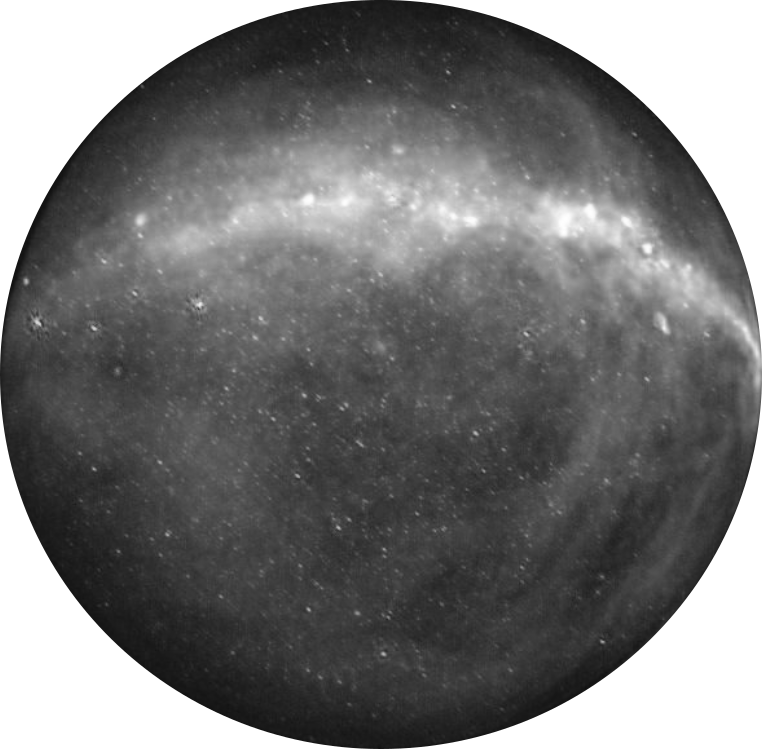
\includegraphics[width=\textwidth]{figures/chapter2/after-expansion}
    \caption{
        Snapshot image of the sky captured with the OVRO-LWA and using the new long-baseline
        antennas. The image covers the entire visible hemisphere in sine-projection.  A similar
        image constructed using only the core of the interferometer can be seen in
        Figure~\ref{fig:core-snapshot-image}.
    }
    \label{fig:expansion-snapshot-image}
\end{figure}

\section{Calibration of a Low-Frequency Interferometer}

The purpose of calibration is to remove the contribution of the antenna and receivers, including any
gain, filters, and propagation effects along the signal path. At low radio frequencies, the Earth's
ionosphere is additionally important due to the effects of electromagnetic waves propagating through
a magnetized plasma.

Further, we will make a distinction between a ``direction-independent'' calibration and a
``direction-dependent'' calibration. The former can correct for the response of the receiver and
signal path, but cannot fully account for the antenna response pattern and ionospheric effects. The
latter allows for the calibration parameters to vary as a function of direction on the sky, which
can account for errors due to the antenna beam and some ionospheric effects.

Neglecting complexity associated with polarized imaging for now, a direction-independent calibration
amounts to determining the complex-valued gain $g_i(\nu)$ associated with each signal path $i$ and
frequency $\nu$. These gains effect the measured correlation between the signal paths $i$ and $j$
such that
\begin{equation}
    V_{ij}^\text{measured}(\nu) = g_i(\nu)\,g_j^*(\nu)\,V_{ij}^\text{true}(\nu)
        + \text{noise}\,,
\end{equation}
where $V_{ij}^\text{measured}$ is the visibility actually measured between the corresponding signal
paths at the frequency $\nu$, and $V_{ij}^\text{true}$ is the visibility that would have been
measured if instead we had correlated the value of the electric field at the electrical center of
each antenna without the need for any additional electronics. The true visibility
can be computed from the sky brightness $I(\nu, \hat{r})$ at the
frequency $\nu$ and direction $\hat r$ such that
\begin{equation}
    V_{ij}^\text{true}(\nu) = \int a_i(\nu, \hat{r})\,a_j^*(\nu, \hat{r})\,I(\nu, \hat{r})\,
        \exp\Big(2\pi i\hat{r}\cdot\vec{b_{ij}}/\lambda\Big)\,\d\Omega,
\end{equation}
where the integral runs over solid angle $\Omega$, $a_i(\nu, \hat{r})$ is the response of the
corresponding antenna at the frequency $\nu$ to the direction $\hat{r}$, $\vec{b_{ij}}$ is the
baseline separating the antennas for signal paths $i$ and $j$, and $\lambda$ is the wavelength.  If
the sky is assumed to be composed of point sources, then
\begin{equation}\label{eq:antenna-response-point-sources}
    V_{ij}^\text{true}(\nu) = \sum_k a_i(\nu, \hat{r}_k)\,a_j^*(\nu, \hat{r}_k)\,F_k(\nu)\,
        \exp\Big(2\pi i\hat{r}_k\cdot\vec{b_{ij}}/\lambda\Big)\,,
\end{equation}
where $F_k$ is the flux of the $k$th point source in the direction $\hat{r}_k$.

A typical calibration strategy using, for example, the Very Large Array (VLA) involves periodically
pointing at a known compact point source. For a compact point source at the phase center, the phase
of all visibilities is zero, and the amplitude is given by the known flux of the source.
Periodically revisiting this source allows for the observer to establish the time variation of the
calibration parameters. Each time the observer solves for the gains that minimize
\begin{equation}
    \chi^2 \propto \sum_{i \neq j}
        \Big\|V_{ij}^\text{measured}(\nu) - g_i(\nu)\,g_j^*(\nu)\,F\Big\|^2\,,
\end{equation}
where $F$ is the flux of the isolated point source.

This optimization can be performed with rapid convergence using a variant of alternating
least-squares developed by \citet{2008ISTSP...2..707M} and \citet{2014A&A...571A..97S}. At each
iteration this algorithm applies linear least-squares to minimize $\chi^2$ while holding one set of
gains constant:
\begin{equation}\label{eq:stefcal-iterations}
    g_i \leftarrow \frac
        {\sum_{i \neq j} g_j^* V_{ij}^{\text{model},*} V_{ij}^\text{measured}}
        {\sum_{i \neq j} \| g_j V_{ij}^\text{model} \|^2}\,,
\end{equation}
where we have now allowed for a more general sky model to be used during calibration by introducing
the model visibilities $V_{ij}^\text{model}$, which are the true visibilities for an assumed model
of the sky.  Naively applying Equation~\ref{eq:stefcal-iterations} will result in poor convergence
due to oscillations about the true minimum of $\chi^2$.  These oscillations can be damped by
averaging subsequent iterations, and \citet{2014A&A...571A..97S} demonstrated that this simple
gradient-free optimization strategy converges remarkably quickly.

The OVRO-LWA is capable of imaging the entire hemisphere in a snapshot image. This brings its own
unique calibration challenges because it is currently impossible to isolate a single compact point source
within the field of view of the interferometer.\footnote{
    Gated pulsar observations could, in principle, achieve this isolation. This capability is a key
    development area for the OVRO-LWA.
}
Due to the wide field of view, determining an accurate gain calibration relies on a detailed sky and
antenna beam model. Mistakes or omissions in the sky model can, for example, generate artificial
ripples in the bandpass that will impact the interferometer's ability to cleanly separate foreground
emission from cosmological 21~cm emission \citep{2016MNRAS.461.3135B, 2017MNRAS.470.1849E}.

Furthermore, at frequencies $\nu < 100\,\text{MHz}$ there are few flux calibrators.
\citet{1977A&A....61...99B} determined the absolute spectrum of Cyg~A between 20~MHz and 2~GHz.
\citet{2012MNRAS.423L..30S} added six additional calibrators, and \citet{2017ApJS..230....7P} used
the VLA 4-band system to bring the total number of available calibrators to 11. However, in
Chapter~\ref{chapter3} I will show that the latter spectra can diverge substantially from truth
below 50~MHz.

Detailed sky and beam models are therefore generally an important calibration requirement for
low-frequency interferometers.  In Chapter~\ref{chapter3}, I will also derive an empirical beam
model for the OVRO-LWA and developed a new imaging formalism that captures the entire visible sky in
a single synthesis imaging step that can be used as part of a self-calibration loop
\citep{1978ApJ...223...25R}.

As part of this thesis I developed the \texttt{TTCal} calibration routine for the purpose of
calibrating the OVRO-LWA. It implements the alternating least-squares algorithm described above to
solve for the complex-valued gain of each signal path from a model sky composed of any number of
point sources, Gaussians, and shapelet components \citep{2003MNRAS.338...35R}. If desired,
\texttt{TTCal} may instead solve for the Jones matrix associated with each antenna for a fully
polarized calibration solution. \texttt{TTCal} is freely available under the GPLv3 license or any
under later version.\footnote{
    \url{https://github.com/mweastwood/TTCal.jl}
}

%Some interferometers (e.g., HERA and the MWA), recognizing the difficulty of gain calibration at low
%frequencies, have opted for partly redundant antenna configurations. These configurations can solve
%for many of their calibration parameters internally without relying on an incomplete sky model and
%potentially inaccurate antenna beam model \citep{2010MNRAS.408.1029L}. However, these
%interferometers sacrifice imaging fidelity, which is useful for establishing the remaining
%calibration parameters (e.g., the overall bandpass cannot be solved for in an internal
%redundant-calibration routine).

\section{Source Removal and Direction-Dependent Calibration}

The large field of view of the OVRO-LWA comes with additional challenges associated with the
ionosphere, inhomogeneous primary beams, and mutual coupling between antennas.

The dispersion relation for electromagnetic waves propagating in a plasma is
\begin{equation}
    \omega^2 = \omega_\text{plasma}^2 + c^2 k^2\,,
\end{equation}
where $\omega$ is the angular frequency of the oscillations, $k$ is the wavenumber, $c$ is the speed
of light, and $\omega_\text{plasma}$ is the plasma frequency---the frequency of electrostatic
oscillations within the plasma. The plasma frequency (in SI units) is given by
\begin{equation}
    \omega_\text{plasma} = \sqrt{\frac{n_e e^2}{m_e \varepsilon_0}}\,,
\end{equation}
where $n_e$ is the number density of electrons, $e$ is the charge of the electron, $m_e$ is the mass
of the electron, and $\varepsilon_0$ is the permittivity of free space.  For Earth's ionosphere, the
plasma frequency is typically $\sim 2\pi \times 10\,\text{MHz}$.  The index of refraction is
\begin{equation}
    n = \sqrt{1 - \frac{\omega_\text{plasma}^2}{\omega^2}}
      \approx 1 - \frac{1}{2}\frac{\omega_\text{plasma}^2}{\omega^2}\,,
\end{equation}
where the approximation holds if $\omega^2 \gg \omega_\text{plasma}^2$. In this regime, the arrival
time of a burst of radio emission is $\propto \nu^{-2}$ as is commonly seen in pulsar astronomy.
The additional phase imparted is, however, $\propto \nu^{-1}$ such that along a given line of sight
the phase can be parameterized as
\begin{equation}
    \phi \approx \phi_0 + \overbrace{2\pi\tau\nu}^\text{delay}
    + \overbrace{\frac{e^2}{4\pi m_e c \varepsilon_0}
        \frac{1}{\nu}\int n_e\,\d l}^\text{ionospheric dispersion}\,,
\end{equation}
where $\phi_0$ sets the overall phase, $\tau$ is the delay, and the integral of the electron number
density along the line of sight is called the Total Electron Content (TEC).

The diffractive scale $r_\text{diff}$ of the ionosphere is the length scale over which the phase
variance is $1\,\text{rad}^2$. The Fresnel scale is $r_\text{f} = \sqrt{\lambda D / 2\pi}$ where $D$
is the height of the ionosphere (typically $\sim 300\,\text{km}$). In the weak scattering regime
($r_\text{diff} \gg r_\text{f}$), the ionosphere can contribute amplitude and phase scintillation,
which may be folded into the antenna gain calibration.  However, in the strong scattering regime
($r_\text{diff} \lesssim r_\text{f}$), point sources may become multiply imaged, which cannot be
described as a perturbation to the antenna response \citep{2015MNRAS.453..925V}.

The antenna response is also generally expected to be inhomogeneous.  Within the core of the
OVRO-LWA antennas are separated by as little as 5\,m.  \citet{2011ITAP...59.1855E} studied the
impact of mutual coupling on the antenna primary beam within the first Long Wavelength Array station
in New Mexico (LWA1), which uses the same antennas and same 5\,m minimum spacing as the OVRO-LWA,
but the antennas are packed within a 100\,m diameter (as opposed to a 200\,m diameter for the
OVRO-LWA). The authors found that, between 20--74\,MHz, when pointing more than
10$\arcdeg$--20$\arcdeg$ from zenith, mutual coupling and correlated galactic noise led to a
2--6\,dB increase in the system equivalent flux density (SEFD), and 1--2\,dB deviations in the
primary beam pattern between antennas. We expect comparable effects for the OVRO-LWA.

Direction-dependent calibration therefore attempts to account for ionospheric scintillation and
refraction, and inhomogeneous antenna beams by allowing the antenna response in
Equation~\ref{eq:antenna-response-point-sources} to be a free parameter.



\texttt{TTCal}







\section{Commissioning Challenges}
\label{sec:commissioning-challenges}

\subsection{Computing Antenna Positions}

\begin{figure}
    \centering
    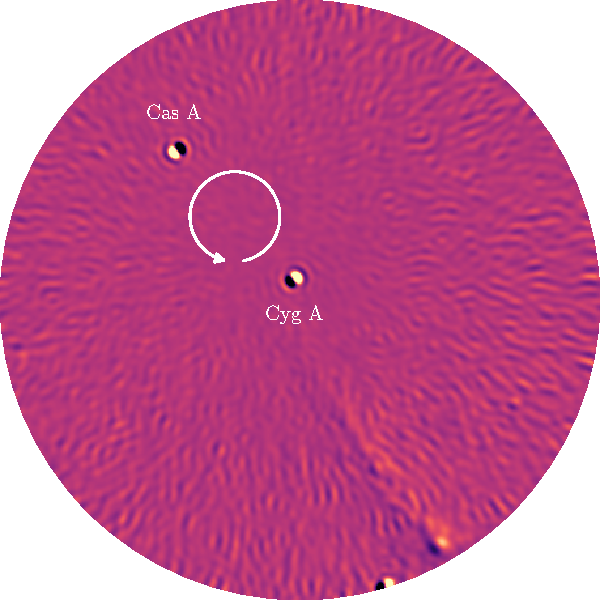
\includegraphics[width=0.7\textwidth]{figures/chapter2/northing-easting-mistake/northing-easting-mistake}
    \caption{
        Illustration of the error in the WCS prior to a correction to the antenna positions. The
        image is a difference between an image constructed with the incorrect antenna positions and
        the corrected antenna positions. The arrow denotes the direction and approximate center of
        the rotation.
    }
    \label{fig:northing-easting-mistake}
\end{figure}

Early images produced by the OVRO-LWA (prior to 2015 October 16) were afflicted by an apparent
rotation in the World Coordinate System (WCS).

\subsection{RFI Localization}

\begin{figure}
    \centering
    \begin{tabular}{cc}
        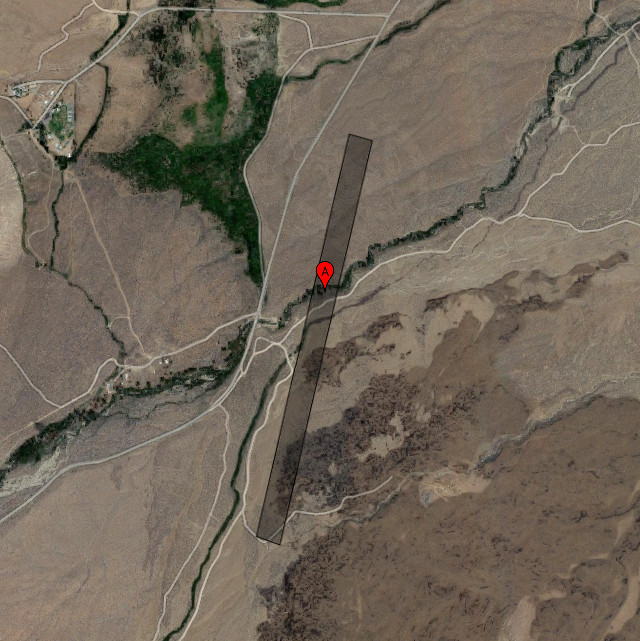
\includegraphics[width=0.45\textwidth]{figures/chapter2/google-maps-rfi-localization} &
        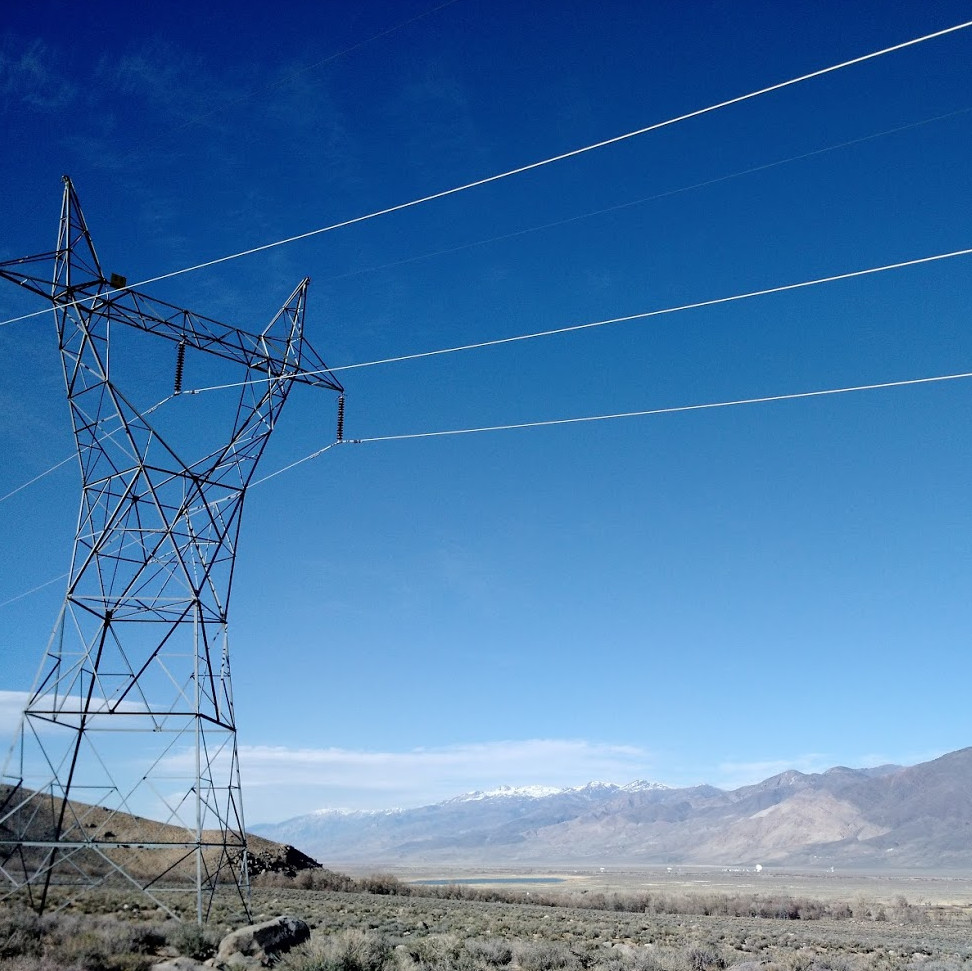
\includegraphics[width=0.45\textwidth]{figures/chapter2/power-line-picture} \\
        (a) & (b) \\
    \end{tabular}
    \caption{
        (a) The localization region for a source of RFI south of the OVRO-LWA and near the town of
        Big Pine. Satellite imagery \textcopyright2018 Google. Map data \textcopyright2018 Google.
        (b) Image of a high-voltage power line overlooking OVRO near the localization region.
    }
    \label{fig:rfi-localization}
\end{figure}

An ongoing challenge faced by the OVRO-LWA is the presence of broadband sources of RFI in the
vicinity of the observatory. Due to the entire-hemisphere field of view of the OVRO-LWA, these
sources appear as points on the horizon that limit the sensitivity of snapshot images through
additional sidelobe noise. Fortunately, because these sources are typically in the near-field of the
interferometer, the curvature of the incoming wavefront can be used to infer the distance to each
source of RFI.

The path difference from a source in the near-field of an interferometer located at the position
$(\xi, \eta, \zeta)$ to two antennas located respectively at $(x_i, y_i, z_i)$ and $(x_j, y_j, z_j)$
is
\begin{equation}\label{eq:nearfield-path-difference}
    \Delta l^\text{near-field}_{ij} =
        \sqrt{(x_j - \xi)^2 + (y_j - \eta)^2 + (z_j - \zeta)^2}
        - \sqrt{(x_i - \xi)^2 + (y_i - \eta)^2 + (z_i - \zeta)^2}\,.
\end{equation}
In the limit that the distance of the source goes to infinity, we recover the familiar expression
\begin{equation}\label{eq:farfield-path-difference}
    \Delta l^\text{far-field}_{ij} = \frac{1}{D}\Big(
        (x_i - x_j)\,\xi + (y_i - y_j)\,\eta + (z_i - z_j)\,\zeta
    \Big)\,,
\end{equation}
where $D$ is the distance to the source. The correlation measured between two antennas for a source
in the near-field of the interferometer is therefore
\begin{equation}\label{eq:nearfield-visibilities}
    V_{ij} = F \exp\left(2\pi i \frac{\Delta l^\text{near-field}_{ij}}{\lambda}\right)\,,
\end{equation}
where $V_{ij}$ is the visibility measured between antennas $i$ and $j$, $F$ is the apparent
brightness of the source, and $\lambda$ is the wavelength. Equation~\ref{eq:nearfield-visibilities}
can then be used to fit for the position of a source including its distance.

In order to improve sensitivity to these RFI sources,



\myputbib{thesis}
\end{bibunit}

